\section{Mission U}
\subsection{Sous-mission U1}

	\begin{vwcol}[widths={0.65,0.2}, rule=0pt]
	\begin{minipage}{0.7\textwidth}
	\paragraph{Objectifs de la mission}

	Mettre en valeur les routes présentes sur l'image. repèrées par un changement brusque de couleur.
	\end{minipage}

	\begin{minipage}{0.3\textwidth}
	\begin{flushright}
	\paragraph{Techniques utilisés}

	Normalisation \& Detection des contours
	\end{flushright}
	\end{minipage}

	\end{vwcol} 

	\begin{figure}[h]
	\centering
		\begin{multicols}{2}
		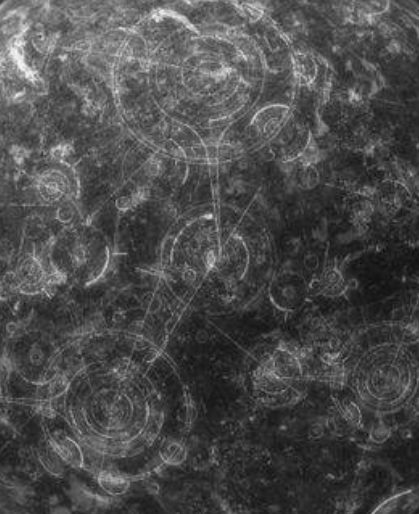
\includegraphics[scale=0.6]{images/U1_surface.png}
		Avant
		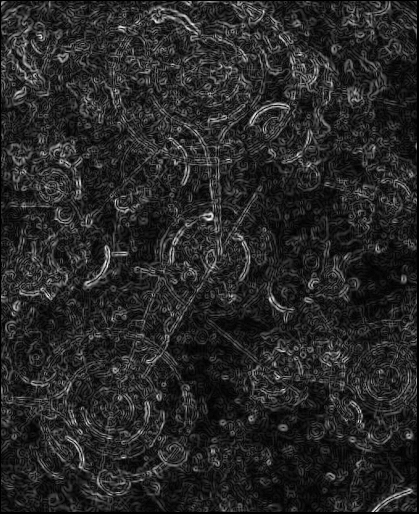
\includegraphics[scale=0.6]{images/MissionU1.png}
		Après
		\end{multicols}
	\end{figure}
	\vspace{-0.9cm}

	\paragraph{Procédé}	
		Pour vérifier la présence des routes, nous avons appliqué un filtre de \emph{detection de contours}. Ce filtre permet de mettre en évidence les contours de l'image et donc les changement brusques de couleur. On applique ensuite un filtre de \emph{normalisation} permettant de rendre l'image plus lisible.